\chapter{Tests}
\label{ch6:tests}

This chapter presents tests carried out in order to verify the proper working of the realised framework. 
%In order to test the developed framework a new hardware was used with a dedicated sensor. 

%Hardware and sensor was provided by Creotech Instruments S.A. which was developing a scientific camera with cooperation with Cracow University
%of Technology. The framework was adapted to the new hardware and acquisition from the dedicated sensor was performed
%using one of the before mentioned techniques. 


\section{Custom Silicon Sensor - Ethernet data transmission}

\subsection{Setup}
\subsection{Test results}


\section{CMV4000 - Serial ATA SSD video data storage}

\subsection{Setup}
The development system was configured with CMV4000 acquisition IP and Serial ATA. The video data correctness was tested
using Ethernet interface which was sensing acquired frames using RTP\footnote{Real-Time Transport} protocol. 

\subsection{Test results}
Video data reception from the CMV4000 CMOSIS sensor was successful. Figure~\ref{PIC:OUTPUT0} presents the acquired image
of the fan which was used for testing the speed of the camera reception.

\begin{figure}[H]
    \centering
    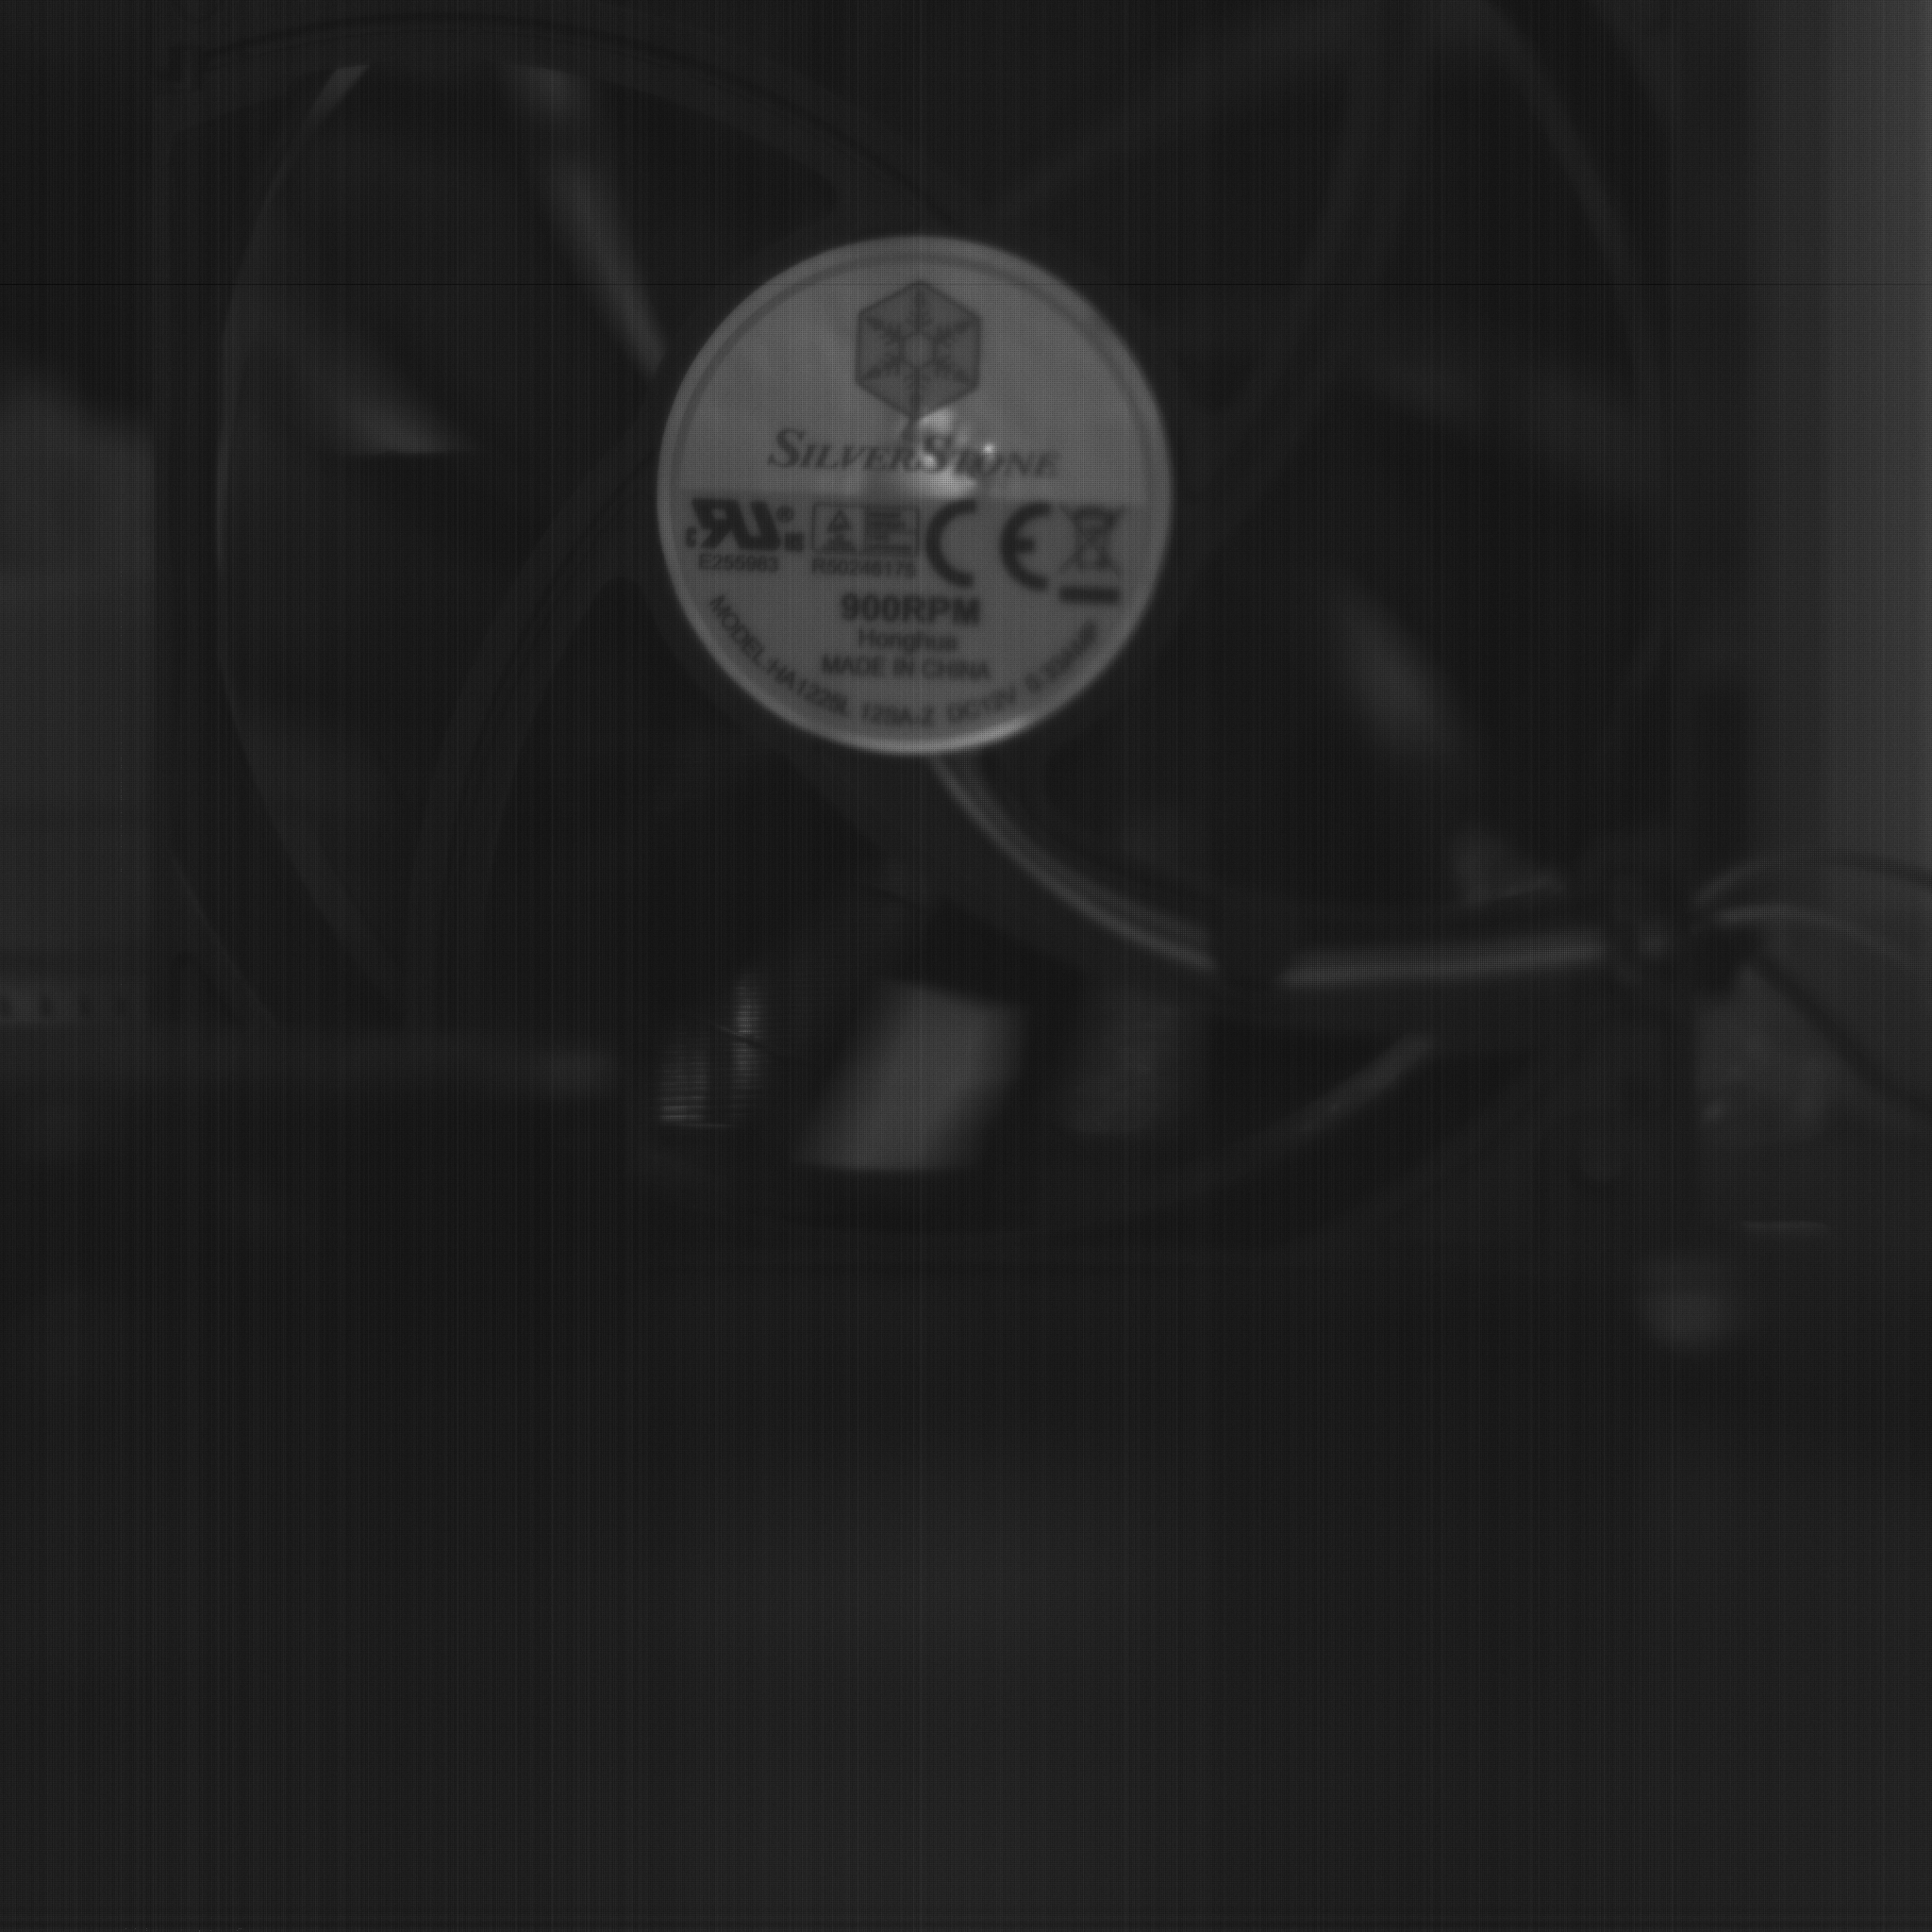
\includegraphics[width=13cm]{img/tests/output0.png}
    \caption{Acquired image from the CMV4000 sensor}
    \label{FIG:OUTPUT0}
\end{figure}


Unfortunately the SSD data acquisition was unreliable. Small portions of data were possible to be written to both of the
hard drives, nevertheless the IP Core constantly lost communication and was resetting itself. As it turned out, the
reason for that was an interal mechanism for sustaining the \textbf{Link-Up} signal high. This signal, when it is high,
indicated that the calibration of the IP Core was successful and that the data can be written or read. The internal
mechanism detected the state of this signal and in a situation where the signal was low, an \textbf{internal reset} was
performed, which \textbf{disrupted} the video data storing. 


\section{Summary}

As far as testing of the camera framework is concerned, the results partially fulfil the requirements, but more work
has to be performed in order to mitigate the limited performance and functionality in some aspects. These limitation
result mainly in wrong assumptions in terms of correctness of operation of some IP Cores which was not possible to
foresee before development. This also underlines a crucial aspect of embedded system design, that before a hypothesis is
not tested and verified, one can not be certain whether some design works or not. 

The most important functions of the framework work correctly and provide a valuable foundation for camera development.  



